\documentclass[11pt]{article}

% Anonymous review version: page numbers + ruler.
\usepackage[review]{acl}

\usepackage{times}
\usepackage{latexsym}
\usepackage[T1]{fontenc}
\usepackage[utf8]{inputenc}
\usepackage{microtype}
% Inconsolata is recommended by ACL for typewriter text. Comment in if available.
% \usepackage{inconsolata}
\usepackage{graphicx}
\usepackage{booktabs}
\usepackage{multirow}
\usepackage{float}      % provides [H] to keep appendix tables next to their text
\usepackage{placeins}   % provides \FloatBarrier so floats stay within their section
\usepackage{amsmath}
\usepackage{amssymb}
\usepackage{xcolor}
\usepackage{xspace}

% Ensure figures are searched in the figures/ subfolder.
\graphicspath{{figures/}}

% Convenience macros.
\newcommand{\sourceall}{\texttt{source\_all}\xspace}
\newcommand{\bestpair}{\texttt{best\_pair}\xspace}
\newcommand{\defsubj}{\texttt{def\_subject}\xspace}
\newcommand{\deftarg}{\texttt{def\_target}\xspace}
\newcommand{\queryword}{\texttt{query\_word}\xspace}
\newcommand{\effect}{\ensuremath{\Delta}\xspace}

\title{Priors Persist Through Suppression: A Stroop Paradigm for Lexical Override}

\author{Anonymous EMNLP Submission}

\begin{document}
\maketitle

\begin{abstract}
Glossaries, technical specifications, and system prompts routinely ask language models to use
familiar words in unfamiliar ways. When this works, the lexical prior persists through
override rather than being replaced: it continues to operate after the local rule applies,
with the rule lowering its logit rather than installing the new meaning on top. We test this
with a Stroop-style paradigm---a remapping rule (\textit{doctor} means \textit{forest}) pitted
against the query word's lexical-prior distractor (\textit{hospital}), with matched neutral
controls. Across $11$ open-weight models spanning four families and $1$B--$9$B parameters,
lexical-prior strength predicts interference even after item-level controls for answer prior,
frequency, tokenization, and prompt wording. Activation patching on five aligned models, on the
antonym-remapping family under a single prompt template, locates a source-position triplet
(definition subject, definition target, query word) that binds the local rule. Dissociation experiments isolate target preservation as the
binding-specific signature: distractor suppression occurs under matched, swap, and
item-mismatched conditions alike, whereas target logit collapse occurs only when the
definition-target position is corrupted. Behavior and mechanism converge on the same channel:
the lexical prior is where both interference originates and where override leaves its mark.
\end{abstract}


% =============================================================================
\section{Introduction}
\label{sec:intro}

Language models are routinely asked to follow local definitions that temporarily change
what familiar words mean. A legal document may define a familiar term in an unusual way; a
technical manual may repurpose a common word as a domain symbol; a system prompt may introduce
a fictional rule. A software glossary defining \emph{port} as a socket still has to fight the
model's prior preference for \emph{harbor}, and the glossary does not always win. These cases require \emph{contextual override}: the model must use the
locally specified meaning while suppressing interference from the word's pretrained lexical
prior. Override failures are quiet---a residual bias toward the prior in next-token
probabilities---but they recur wherever local-definition fidelity matters, from glossary
lookup to retrieval-augmented document grounding.

Contextual override against lexical priors is \emph{not} a clean replacement of meaning. It
is a competition. The prior keeps operating, and its strength still shows through. This makes
two predictions. Items whose distractor is more strongly favored by the model's ordinary
lexical prior should show larger interference, even after surface controls. And a causal
intervention that recovers override should change the target--distractor margin
asymmetrically along the lexical-prior \emph{channel}---the axis $\log P(t) - \log P(d)$ at
the readout position, where prior interference manifests.

We test these claims with a Stroop-style paradigm (Figure~\ref{fig:paradigm}). A prompt remaps
a query word $w$ to a contextual target $t$; a matched neutral control prompt replaces $w$
with a semantically weak word but holds the target and a competing lexical-prior distractor
$d$ fixed. The target--distractor pair is identical in surface form and tokenization across
conditions; only the query word changes by design, and the residual surface differences this
introduces are absorbed by item-level covariates. The structure mirrors the classic
\citet{stroop1935} task, in which a task-relevant dimension (the contextual mapping) is
pitted against an automatic but irrelevant one (the lexical prior).

\begin{figure}[t]
\centering
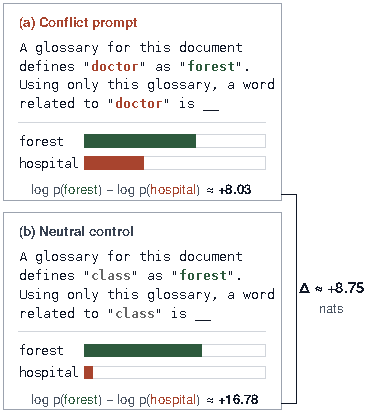
\includegraphics[width=0.85\columnwidth]{fig1_paradigm.pdf}
\caption{The Stroop-style paradigm. Conflict prompt: \emph{doctor means forest} with target
\emph{forest} and lexical-prior distractor \emph{hospital}. Neutral control: query word
replaced by \emph{class} (one of six sampled neutrals). Numbers are sum log-probabilities of
target and distractor under Gemma-2-2B-Instruct (glossary prompt); $\effect$ is neutral minus
conflict $\log P(t) - \log P(d)$ (\S\ref{sec:paradigm}). Displayed neutral gives
$\effect \approx 8.75$; six-control mean $\approx 8.61$.}
\label{fig:paradigm}
\end{figure}

Behaviorally, across $11$ open-weight models spanning the Qwen, Gemma, OLMo, and Mistral
families and four prompt styles, aggregate interference is positive in every model and in
every conflict family. The effect is smallest for the canonical Stroop case (antonym
remapping) and $2$--$4\times$ larger for the document-relevant families (arbitrary, polysemy,
domain-definition)---the settings where lexical override matters in practice. After item-level
controls for answer prior, frequency, tokenization, prompt style, conflict family, model
family, scale, and instruction tuning, the distractor's lexical-prior strength remains a
positive predictor of interference, and the coefficient holds its sign under item-clustered,
model-clustered, two-way clustered, and mixed-effects standard errors. Priors leak through
override in proportion to their strength rather than being erased by the local rule.

Mechanistically, on a tractable subset of five aligned models, residual-stream activation
patching identifies a \emph{source triplet} (the joint representation of the definition
subject, definition target, and query word) whose recovery exceeds every source-position pair
at the site and layer the triplet selects for that model. Held-out splits, item-mismatched
source controls, a definition-target swap that preserves the identity match while corrupting
only the local-value position, and reader-component zero-ablation all support a binding
interpretation. A logit decomposition then shows that the triplet intervention raises the
target--distractor margin asymmetrically: the distractor logit drops under matched, swap, and
item-mismatched conditions alike, while the target logit is preserved only under matched
binding. Distractor suppression marks where override repair (the patch-induced restoration of the
target--distractor margin under matched binding) lands in the logit channel; target
preservation is binding's specific contribution.

Our contribution is not the observation that LMs sometimes fail to override priors; this has
been documented at the benchmark, demonstration, and entity-conflict levels. It is the
convergence: a single lexical-prior channel that both predicts which items resist override
behaviorally and absorbs the causal effect of override repair mechanistically. Two
independent measurements---an item-level behavioral predictor and a position-level causal
intervention---land on the same target--distractor axis.

Concretely, this paper contributes: (i) a controlled Stroop-style paradigm for lexical-level
override, with matched neutral baselines that isolate lexical-prior interference per item;
(ii) evidence across $11$ open-weight models that lexical-prior strength predicts override
failure even after item-level controls for answer prior, frequency, tokenization, and prompt
wording; (iii) a mechanistic dissociation in which the source-position triplet recovers the override
effect, with the binding-specific logit signature localizing to the definition-target position
alone: distractor suppression occurs broadly under source-position perturbation, but target
logit collapse occurs only when the definition-target position is corrupted. Behavior and
mechanism converge on the same channel.


% =============================================================================
\section{Related Work}
\label{sec:related}

\paragraph{Conflicts between context and parametric knowledge.}
A growing body of work studies how language models reconcile in-context information with
information memorized at pretraining \citep{longpre2021entity, xie2024knowledge,
kortukov2024studying}, with \citet{xu2024knowledge} surveying context--memory, inter-context,
and intra-memory conflicts. Almost all of this work operates at the document or claim level
(entity reassignment, passage contradiction) and reads the model's open generation. Our
setting is lexical-level; the readout is a teacher-forced target-versus-distractor margin,
not free generation; and every conflict prompt has a matched neutral remapping that holds the
target/distractor pair fixed, so lexical-prior interference from the query word reads off
directly. Concurrent benchmark-level work documents semantic-override failures on logic and
circuit reasoning tasks \citep{thota2026semantic}; we focus instead on a controlled
lexical paradigm that yields a per-item behavioral predictor and a position-level mechanistic
readout.

\paragraph{Psycholinguistic probes of lexical interference.}
Earlier probes measure lexical interference without Stroop framing:
\citet{ettinger2020bert} adapts cloze diagnostics to pretrained models;
\citet{kassner2020negated} show that a misleading prime drags masked-token predictions toward
the prime; \citet{misra2020priming} find that semantic priming in BERT flips to interference
under stronger sentential constraint. Our conflict is induced by an explicit local definition
rather than a freestanding prime, each prompt has a matched \emph{neutral remapping} that
preserves the target/distractor pair, and scoring is over a target-minus-distractor margin.
Matched baselines turn lexical-prior advantage into a quantitative item-level predictor of
interference (\S\ref{sec:behavior}). Our Stroop analogy is methodological---matched neutral
controls and factorial design---not a claim that the LM's lexical prior is a competing
percept in the cognitive sense.

\paragraph{In-context learning and prior tug-of-war.}
\citet{wei2023larger} and \citet{pan2023incontext} document a tension between
\emph{task recognition} from priors and \emph{task learning} from demonstrations, with scale
and instruction tuning shifting the balance; \citet{shi2023distracted} show that irrelevant
context pulls predictions away from the prior. Our paradigm is a sharper microcosm: a single
in-prompt rule replaces multi-shot demonstration, a binary lexical readout replaces task
accuracy, and prior strength is measured directly per item rather than inferred from
population-level base-rates.

\paragraph{Mechanistic interpretability of knowledge conflicts.}
Activation patching \citep{vig2020causal, meng2022rome, zhang2024towards} and circuit-level
analyses \citep{wang2023ioi, olsson2022induction, mcdougall2024copy} localize internal
representations causally, with copy suppression \citep{mcdougall2024copy} establishing that
attention heads can shape outputs by lowering wrong-token logits rather than by writing
correct ones. Within knowledge conflicts specifically, \citet{yu2023characterizing},
\citet{ortu2024competition}, and \citet{jin2024cutting} identify attention heads that promote
memorized versus in-context answers at the document and entity level, with the individual
head as the unit of analysis. A parallel line on in-context binding
\citep{feng2024binding, prakash2024finetuning, gurarieh2025mixing} studies how LMs
retrieve bound entity--attribute pairs in general. We ask a different question on a different
unit: how a single in-prompt lexical redefinition competes with a word's pretrained prior,
with a source-position triplet---definition subject, definition target, query word---as the
unit of analysis. Unlike entity--attribute binding where the attribute is explicit context
content, our redefinition binds an existing-meaning token to a new contextual value while the
prior meaning remains a strong competing completion.

Two concurrent strands are particularly close. \citet{thota2026semantic} document
override failures at the benchmark level on logic and circuit reasoning, complementing our
controlled lexical paradigm and mechanistic readout. \citet{ma2026corect} report a layer-wise
parametric suppression in which deeper layers progressively overwrite retrieved context with
pretrained answers; we find a position-level dual in the override-success direction. At the
position level, distractor suppression is patch-broad rather than binding-specific: it
occurs under any source-position perturbation, while binding's distinctive contribution is
selective target preservation (\S\ref{sec:robustness},
Table~\ref{tab:logit_decomp_all}). Together with copy suppression at the head level, these
results situate suppression as a patch-broad channel through which LMs modulate competing
predictions, separable from the binding-specific channel that protects the contextual target.

\paragraph{Binding and representation engineering.}
\citet{feng2024binding} identify a binding-ID mechanism pairing entities to attributes via
low-rank vectors, and \citet{prakash2024finetuning} show that entity tracking shares its
circuit across LLaMA fine-tunes. Our triplet binds a query word to its locally redefined
meaning rather than an entity to its properties; the definition-target swap
(\S\ref{sec:mechanism}) directly tests this binding. Representation-engineering methods
\citep{turner2023activation, zou2023representation, hernandez2024inspecting} act on the model
side via fixed steering or edit directions; our intervention acts on the data side, patching
the clean activation from the same item back into the corrupted run.


% =============================================================================
\section{The Semantic Stroop Paradigm}
\label{sec:paradigm}

\subsection{Stimuli}

Each item specifies a query word $w$, a lexical-prior distractor $d$, and a context-defined target $t$.
The conflict prompt remaps $w$ to $t$ inside a wrapper sentence; the neutral prompt replaces $w$ with
a semantically weak word $n$ chosen from a neutral pool, while leaving $t$ and $d$ unchanged
(Figure~\ref{fig:paradigm}). The glossary wrapper renders the running \emph{doctor} item as
\texttt{A glossary for this document defines "doctor" as "forest". Using only this glossary,
a word related to "doctor" is}, with $t={}$\emph{forest}, $d={}$\emph{hospital}; the neutral
prompt substitutes a neutral $n$ for \emph{doctor}. The relation cue is family-specific (\texttt{a synonym of} for antonym,
\texttt{a word related to} for the other three; Appendix~\ref{app:stimuli},
Table~\ref{tab:prompt_templates}). Target and distractor completions are identical in surface
form and tokenization across conditions; the query word varies by design. We average over
multiple neutral words per item and include token-count and frequency covariates in the
controlled regression to absorb residual length and surface effects.

\paragraph{Conflict families.}
We evaluate four families that span psycholinguistic and document-style settings:
\textbf{(i)} \emph{antonym remapping} (\emph{small means big}; the original Stroop analogue);
\textbf{(ii)} \emph{arbitrary semantic remapping} (\emph{apple means river}); \textbf{(iii)}
\emph{polysemy/entity remapping} (\emph{jaguar means car}); and \textbf{(iv)}
\emph{domain-definition remapping} (\emph{thread means process}). Per-family examples in
Table~\ref{tab:stim_examples}.

\paragraph{Prompt styles.}
Each item is rendered under four wrappers: game-rule (toy framing), glossary (document
glossary), technical-document (technical convention), and scoped-definition (passage-scoped
rule); full templates in Table~\ref{tab:prompt_templates}. This tests whether interference is
tied to toy wording or persists in document-like settings.

\subsection{Behavioral metric}

For prompt $x$, let $S(x) = \log P(t \mid x) - \log P(d \mid x)$ denote relative target preference,
where $P(\cdot \mid x)$ is the model's full-sequence probability under teacher forcing.
The Stroop-style interference effect is
\[
\effect = \mathbb{E}_{n \in \mathcal{N}}\!\left[ S(x_{\text{neutral},n}) \right] - S(x_{\text{conflict}}),
\]
where $\mathcal{N}$ is the set of sampled neutral controls for the item.
Positive \effect~means lexical conflict reduces relative target preference.
We report sum log-probability as the primary metric; mean per-token log-probability gives a
length-normalized diagnostic that yields the same aggregate model-level and controlled-regression
conclusions, while individual model$\times$family and model$\times$style cells can shift modestly
between the two scoring modes.

\paragraph{Worked example.}
For the running \emph{doctor} item (Figure~\ref{fig:paradigm}; Gemma-2-2B-Instruct under the
glossary wrapper, sum log-probability), $S(x_{\text{conflict}}) \approx {+}8.03$. The displayed
neutral control using \emph{class} gives $S(x_{\text{neutral,\,class}}) \approx {+}16.78$ and
a single-control $\effect \approx 8.75$; the item-level metric averages over six neutral
controls, giving mean $S(x_{\text{neutral}}) \approx {+}16.64$ and $\effect \approx 8.61$.

\paragraph{Lexical-prior strength.}
We measure the strength of the distractor's lexical prior with an
\emph{ordinary-prior prompt} (e.g., \emph{a word related to doctor is}) that contains no
remapping rule. The relation cue matches the family of the conflict prompt (\emph{a synonym
of} for the antonym family, \emph{a word related to} for the other three), so the prior is
measured under the same relation phrase the conflict prompt uses. The lexical-prior advantage
of the distractor over the target is $\log P(d) - \log P(t)$ under that prompt, computed per
item per model; we use this quantity as our operational measure of lexical-prior strength.

\subsection{Models}

The behavioral analysis evaluates $11$ open-weight model settings: Qwen2.5-1.5B and 7B base/instruct
\citep{yang2024qwen25}, Gemma-2-2B and 9B base/instruct \citep{riviere2024gemma2},
OLMo-1B \citep{groeneveld2024olmo}, and Mistral-7B base/instruct \citep{jiang2023mistral}.
We abbreviate the instruction-tuned variants as ``-IT'' in figures and tables.
Mechanistic analysis uses the aligned tractable subset for which full activation patching with
TransformerLens \citep{nanda2022transformerlens} is computationally feasible:
Qwen2.5-1.5B base/IT, Gemma-2-2B base/IT, and OLMo-1B (Table~\ref{tab:model_set}).


% =============================================================================
\section{Behavioral Results}
\label{sec:behavior}

\subsection{Interference is positive across modern models}

\begin{figure}[t]
\centering

\includegraphics[width=\columnwidth]{fig2_model_forest.pdf}
\caption{Model-level Stroop interference \effect~with bootstrap $95\%$ confidence intervals
(sum log-probability scoring). All $11$ evaluated model settings are positive at the aggregate
level, including $7$B/$9$B-class models from four families.}
\label{fig:forest}
\end{figure}

\begin{figure*}[t]
\centering

\includegraphics[width=\textwidth]{fig3_heatmaps.pdf}
\caption{External validity. \textbf{(a)} Effect by conflict family across models.
\textbf{(b)} Effect by prompt style across models. The effect is positive in every family;
the document-relevant families (arbitrary, polysemy, domain-definition) produce larger and
less model-sensitive effects than antonym remapping (the canonical Stroop analogue). The
effect is robust under glossary, technical-document, and scoped-definition wrappers. Cell
values are sum log-probability \effect.}
\label{fig:heatmaps}
\end{figure*}

All $11$ settings have positive aggregate effects (Figure~\ref{fig:forest}), with effect sizes
ranging from $1.31$ (Gemma-2-9B-IT) to $2.71$ (Qwen2.5-7B). Interference is not specific to
small models, to a single family, or to a single training regime.

\subsection{The effect generalizes across conflict families}

The effect is positive in every family. Antonym remapping---the closest psycholinguistic
analogue of a Stroop conflict---holds in every model but at the lowest aggregate level
($\effect = 1.16$, $95\%$~CI $[1.06, 1.26]$, $n{=}3520$; Figure~\ref{fig:heatmaps}(a)); the
three document-relevant families are $2$--$4\times$ larger: arbitrary semantic remapping
$3.97$\,$[3.79, 4.15]$, polysemy/entity $2.66$\,$[2.49, 2.84]$, domain-definition
$2.54$\,$[2.37, 2.73]$ (per-cell values in Table~\ref{tab:model_x_family}). The antonym
minimum is concentrated in the largest instruction-tuned models (Qwen2.5-7B-IT, Gemma-2-9B-IT),
consistent with a relation-phrase-specific confound: antonym prompts use a synonym-seeking cue
(\texttt{a synonym of}) that may activate IT models' specialized opposite-word routines,
whereas the other three families use a broader \texttt{a word related to} cue and are
unaffected (Limitations). The paradigm generalizes to document-grounding settings where lexical override matters:
glossary lookup, polysemous-entity disambiguation, and domain-specific redefinition.

\subsection{The effect persists under document-style wrappers}

Interference survives reframing the conflict as a glossary entry, a technical convention, or a
passage-scoped definition. The game-rule wrapper yields the largest aggregate effect ($3.15$),
but glossary ($2.06$), technical-document ($1.75$), and scoped-definition ($1.94$) wrappers all
remain substantial (Figure~\ref{fig:heatmaps}(b); per-cell values in
Table~\ref{tab:model_x_style}). Of $44$ model$\times$style cells, $42$ have CI $> 0$.

\subsection{Lexical-prior strength predicts interference}
\label{sec:lexical_predictor}

\begin{figure}[t]
\centering

\includegraphics[width=\columnwidth]{fig4_lexical_prior.pdf}
\caption{Lexical-prior strength predicts Stroop interference at the item$\times$prompt level.
Light points: $2{,}500$ subsampled item$\times$prompt observations across all $11$ models.
Open circles: decile means with $\pm 1$\,SE bars. Red line: bivariate OLS fit
($n{=}7{,}744$). The controlled regression in Table~\ref{tab:regression} retains a positive
coefficient after adding answer prior, tokenization, frequency, prompt style, conflict family,
model family, scale, and instruction tuning.}
\label{fig:lexical}
\end{figure}

If interference reflects lexical-prior conflict rather than incidental confounds, then items
whose distractor is more strongly favored by the model's ordinary lexical prior should show
larger \effect. They do (Figure~\ref{fig:lexical}). Pooling all $11$ models at the
item--prompt level, bivariate OLS gives a slope of $0.086$ ($p < 10^{-9}$), and binned decile
means trace a clear monotone trend. In nat units, a one-nat increase in the distractor's
lexical-prior advantage raises Stroop interference by about $0.1$ nat; lexical-prior advantage
ranges over more than $20$ nats across items (Figure~\ref{fig:lexical}), so the predicted
effect spans the full observed range of $\effect$.

\begin{table}[t]
\centering
\scriptsize
\setlength{\tabcolsep}{3pt}
\begin{tabular*}{\columnwidth}{@{\extracolsep{\fill}}lrrr@{}}
\toprule
Term & Coef. & $95\%$ CI & $p$ \\
\midrule
Intercept                 & $+0.746$ & $[+0.38, +1.11]$ & $5.5{\cdot}10^{-5}$ \\
Lexical advantage         & $+0.114$ & $[+0.08, +0.15]$ & $4.5{\cdot}10^{-10}$ \\
Answer prior              & $+0.16$ & $[+0.11, +0.21]$ & $7.7{\cdot}10^{-11}$ \\
Frequency ($\Delta$ zipf) & $+0.65$ & $[+0.43, +0.86]$ & $7.9{\cdot}10^{-9}$ \\
Token-count $\Delta$      & $-0.08$ & $[-0.46, +0.31]$ & $0.69$ \\
Is instruct               & $-0.74$ & $[-1.00, -0.47]$ & $4.0{\cdot}10^{-8}$ \\
$\log$ params (B)         & $-0.32$ & $[-0.44, -0.19]$ & $4.3{\cdot}10^{-7}$ \\
\bottomrule
\end{tabular*}
\caption{Main controlled regression of item$\times$prompt Stroop interference under sum
log-probability scoring ($n{=}7{,}744$). The model also includes fixed effects for conflict
family, prompt style, and model family (omitted for space; see Appendix~\ref{app:regression}).
The intercept and lexical-advantage coefficient remain positive in the main controlled
specification.}
\label{tab:regression}
\end{table}

Table~\ref{tab:regression} reports the controlled OLS regression.
After accounting for answer prior, frequency, tokenization, prompt style, conflict family,
model family, scale, and instruction tuning, the lexical-advantage coefficient remains positive
($+0.114$, $p < 10^{-9}$) and the intercept remains positive ($+0.746$, $p < 10^{-4}$).
The instruct and $\log$-parameter coefficients are negative, indicating that instruction tuning
and scale \emph{reduce}, but do not eliminate, interference.

Standard errors in the main table are clustered by item. The positive lexical-prior advantage
coefficient retains the same sign under clustering by model, two-way clustering by item and
model, and a linear mixed-effects specification with item- and model-level random effects; the
mixed-effects $95\%$ CI lower bound ($+0.014$) is close to zero, so the result is best read as a
\emph{stable positive sign across specifications} rather than as equally tight inference under
all specifications. These robustness results are summarized in Appendix~\ref{app:regression} and
released with the data package. The instruction-tuning and scale coefficients retain the same
negative sign, although their uncertainty increases under model-level and mixed-effects
specifications.

The covariate set is conservative: answer-prior captures whether the target is easier than the
distractor independent of context, and template and architecture shifts are removed by the
fixed effects for prompt style, conflict family, and model family. Lexical-prior advantage remains predictive after all of these---the pattern expected if
interference is driven specifically by the ordinary meaning of the query word. Within the
antonym family alone, the per-item slope is not significant
($+0.026$, $p=0.235$; Table~\ref{tab:regression_interactions}); the pooled coefficient is
carried by the three document-relevant families.


% =============================================================================
\section{Mechanistic Analysis}
\label{sec:mechanism}

The behavioral effects above are broad and not reducible to surface confounds; we now ask
how the conflict is resolved internally.

\paragraph{Scope.}
Mechanistic experiments use the original antonym-remapping family, the game-rule prompt
wrapper, and the single-token subset, on five aligned tractable models for which
TransformerLens loading is reliable.

\subsection{Activation patching setup}

For each item we construct a clean prompt (neutral remapping) and a corrupted prompt
(lexical-conflict remapping) sharing the same target and distractor. We patch clean
residual-stream activations into corrupted runs at three source positions---the
\emph{definition subject} (e.g.\ \emph{small}), the \emph{definition target}
(e.g.\ \emph{big}), and the \emph{query word}---and at the \emph{full source triplet}
combining all three, reporting the standard normalized recovery $R$ of
\citet{zhang2024towards} on the final-position target-minus-distractor logit difference.
Mechanistic items use the single-token target/distractor subset; Appendix~\ref{app:mech_impl}
gives the implementation details.

\subsection{The source triplet binds the local definition}

\begin{figure*}[t]
\centering

\includegraphics[width=\textwidth]{fig5_mechanism_core.pdf}
\caption{Source-triplet residual mechanism.
\textbf{(a)} Layer-wise patching recovery for each source group on Gemma-2-2B at the
residual-stream site the full triplet selects (mid-block). The full triplet sits above every
singleton and pair through mid-network depths.
\textbf{(b)} Recovery for the full triplet versus the best source-position pair across the
five mechanism models, evaluated at the site and layer the triplet selects in each model. The
triplet exceeds the best pair without exception ($\Delta R \in [+0.11, +0.36]$);
split-validation evidence is in the text.}
\label{fig:mechcore}
\end{figure*}

\begin{table}[t]
\centering
\scriptsize
\setlength{\tabcolsep}{3pt}
\begin{tabular*}{\columnwidth}{@{\extracolsep{\fill}}lllrrr@{}}
\toprule
Model & Site & $L$ & $R_{\text{trp}}$ & $R_{\text{pair}}$ & $\Delta R$ \\
\midrule
Qwen2.5-1.5B    & input     & 3  & $0.99$ & $0.89$ & $+0.11$ \\
Qwen2.5-1.5B-IT & input     & 15 & $0.92$ & $0.59$ & $+0.33$ \\
Gemma-2-2B      & mid-block & 12 & $1.05$ & $0.69$ & $+0.35$ \\
Gemma-2-2B-IT   & input     & 3  & $1.04$ & $0.68$ & $+0.36$ \\
OLMo-1B         & input     & 2  & $1.06$ & $0.87$ & $+0.19$ \\
\bottomrule
\end{tabular*}
\caption{Source-triplet residual patching versus the best source-position pair. Site
(residual-stream location: input = block input, mid-block = post-attention) and $L$ (layer)
are selected by the full source triplet; $R_{\text{trp}}$ is the recovery of the full triplet
at that site/layer, and $R_{\text{pair}}$ is the recovery of the best source-position pair at
the same site/layer. The best pair is consistently definition subject + query word; adding
the definition target improves point-estimate recovery in all five models.}
\label{tab:mechsummary}
\end{table}

Joint patching of the definition subject, definition target, and query word recovers more of
the conflict effect than any source-position pair, at the residual-stream site and layer the
triplet selects (Figure~\ref{fig:mechcore}, Table~\ref{tab:mechsummary}). The triplet--pair
margin $\Delta R = R_{\text{triplet}} - R_{\text{pair}}$ falls between $+0.11$ and $+0.36$ in
5/5 models. The best pair is consistently definition subject + query word; adding the
definition target improves recovery at the same site and layer. Recovery for every source
group at this site/layer is in Appendix~\ref{app:mech_extra},
Table~\ref{tab:source_group_recovery}.

Structurally, subject and query supply the identity match while definition target supplies
the local value; $\Delta R$ measures the cost of any missing slot.

\paragraph{Definition-target swap control.}
A definition-target swap tests this directly: keep subject and query word matched, replace
only the definition-target activation with a donor item's. Recovery drops sharply
(matched$-$swap margin $+1.54$ to $+5.26$; Appendix~\ref{app:mech_extra},
Table~\ref{tab:swap_summary}), preserving the identity match while corrupting only the
local-value position. This rules out a purely identity-based account.

\paragraph{Split validation.}
Across $200$ discovery/held-out splits, the held-out triplet--pair margin has a positive mean
in each of the five models---tightly so in base models ($0.97$--$1.00$ positive fraction) and
more heterogeneously in instruction-tuned ones ($0.83$--$0.95$). Per-model values are in
Appendix~\ref{app:mech_extra}, Table~\ref{tab:split_summary}.

\subsection{Binding's logit signature: target preservation, not distractor suppression}

Recovery requires the full triplet ($\Delta R = +0.11$ to $+0.36$ over the best pair, $5/5$
models; Table~\ref{tab:mechsummary}). At the logit-margin resolution, however, the
binding-specific signature localizes to the \texttt{def\_target} position alone: corrupting
\texttt{def\_target} via swap produces a logit decomposition nearly identical to fully
item-mismatched controls (Table~\ref{tab:logit_decomp_all}; $|\Delta m_S - \Delta m_R| \leq 0.6$
nat across all five models).

\begin{table*}[t]
\centering
\scriptsize
\setlength{\tabcolsep}{3pt}
\begin{tabular*}{\textwidth}{@{\extracolsep{\fill}}lrrrrrrrrr@{}}
\toprule
& \multicolumn{3}{c}{Matched (M)} & \multicolumn{3}{c}{Swap (S)} & \multicolumn{3}{c}{Random (R)} \\
\cmidrule(lr){2-4} \cmidrule(lr){5-7} \cmidrule(lr){8-10}
Model & $\Delta\ell_t$ & $\Delta\ell_d$ & $\Delta m$ & $\Delta\ell_t$ & $\Delta\ell_d$ & $\Delta m$ & $\Delta\ell_t$ & $\Delta\ell_d$ & $\Delta m$ \\
\midrule
Qwen2.5-1.5B    & $-1.39$ & $-3.13$  & $+1.74$ & $-12.79$ & $-5.34$  & $-7.45$ & $-12.68$ & $-5.41$  & $-7.27$ \\
Qwen2.5-1.5B-IT & $-6.97$ & $-11.05$ & $+4.08$ & $-16.48$ & $-13.70$ & $-2.77$ & $-16.26$ & $-13.34$ & $-2.91$ \\
Gemma-2-2B      & $+0.17$ & $-3.72$  & $+3.89$ & $-8.04$  & $-6.02$  & $-2.03$ & $-7.95$  & $-5.81$  & $-2.14$ \\
Gemma-2-2B-IT   & $-1.78$ & $-5.60$  & $+3.83$ & $-16.92$ & $-8.03$  & $-8.89$ & $-15.69$ & $-7.40$  & $-8.30$ \\
OLMo-1B         & $-1.38$ & $-3.41$  & $+2.03$ & $-7.68$  & $-5.50$  & $-2.19$ & $-7.56$  & $-5.33$  & $-2.23$ \\
\bottomrule
\end{tabular*}
\caption{Logit decomposition under three patching conditions. M = matched triplet,
S = definition-target swap, R = item-mismatched control. $\Delta m = \Delta\ell_t -
\Delta\ell_d$. Distractor drops comparably across all three (within $0.7$ nat in S vs R);
target collapses only when binding is disrupted. Margin gaps
$|\Delta m_S - \Delta m_R| \leq 0.6$ nat across all five models.}
\label{tab:logit_decomp_all}
\end{table*}

Matched binding preserves the contextual target logit near baseline ($\Delta\ell_t \in
[-7, +0.17]$) while the distractor drops by $3$ to $11$ nats. Under swap and item-mismatched
controls the distractor drops by $5$ to $13$ nats (a comparable order of magnitude, somewhat
larger than matched), but the target collapses by $7$ to $17$ nats, inverting the margin. The
binding-specific signature is therefore selective target preservation; distractor suppression
operates broadly under any source-position perturbation (\S\ref{sec:robustness}).

\subsection{Robustness: item-mismatched controls and reader mediation}
\label{sec:robustness}

\begin{figure}[t]
\centering

\includegraphics[width=\columnwidth]{fig7_evidence.pdf}
\caption{Matched triplet recovery (colored diamond) versus $50$ item-mismatched clean-source
controls (grey points; horizontal bar at the control mean) per mechanism model. Item-mismatched
clean activations \emph{do not} recover the effect; they actively harm it, establishing that
recovery requires item-matched source information. Reader-component mediation summary is in
Appendix~\ref{app:mech_extra}, Table~\ref{tab:mediation}.}
\label{fig:evidence}
\end{figure}

Item-mismatched clean source activations yield strongly \emph{negative} recovery
($-0.58$ to $-4.16$; Figure~\ref{fig:evidence}, Table~\ref{tab:random_summary}); no
perturbation overlaps the matched value, so recovery requires item-matched information.
Zero-ablating top reader components during the matched triplet patch reduces recovery by
$0.19$ to $0.62$ across the five models (Appendix~\ref{app:mech_extra},
Table~\ref{tab:mediation}).


% =============================================================================
\section{Discussion}
\label{sec:discussion}

Two independent measurements landed on the same lexical-prior channel. Behaviorally, a
one-forward-pass estimate of distractor-versus-target prior strength predicts per-item
override interference across $11$ open-weight models, after item-level controls, and across
four prompt wrappers including the document-style framings (glossary, technical, scoped) that
most resemble production use. Mechanistically, a source-position triplet recovers the
override effect; the lexical-prior distractor channel that the behavioral predictor
identifies is also where override repair lands at the logit level. The convergence is the point: the prior is not just where interference comes from,
it is where repair lands.

The mechanistic picture is partial but coherent. A source-position triplet recovers more of
the conflict effect than any pair, and a definition-target swap shows the triplet is doing
binding work rather than identity matching. Writers are distributed and the strongest reader
differs by model; the shared structural pattern is triplet over pair and asymmetric logit
movement at the matched condition.

The logit decomposition revealed a functional partition we did not expect. Matched binding's
contribution to the target--distractor margin runs almost entirely through target
preservation: the distractor logit drops by comparable magnitude under structured corruption
(swap) and unstructured corruption (item-mismatched random), so distractor suppression is a
broad effect of source-position perturbation rather than a binding-specific function. Where
logit-difference recovery is used to identify binding-specific mechanisms, distractor
suppression alone is therefore insufficient; the target channel under binding-violating
controls is the more diagnostic signal.

Across paradigm, behavior, and mechanism, lexical override emerges as a partial competition
rather than a clean substitution. The prior continues to operate; behavioral interference
scales with its strength; and at the position level the same prior channel carries both
interference and its repair, with binding's specific contribution cleanly separable from
broader source-position effects. The Stroop paradigm anchors per-item measurement; the
lexical-prior predictor connects behavior to mechanism; the dissociation isolates which logit
channel signals binding.

\section*{Limitations}

The paradigm is deliberately controlled. Even with glossary, technical-document, and
scoped-definition wrappers, our prompts are shorter than realistic long-form documents, and
the items use English stimuli with target-vs-distractor likelihood scoring rather than
unconstrained free generation.

The mechanistic analysis covers five aligned $1$B--$2$B models where full residual and
component patching is tractable, while the behavioral analysis spans $1$B--$9$B across four
families. Whether the source-triplet structure persists at $7$B$+$ scale, across the four
conflict families, and across non-game-rule wrappers is open; the mechanism is established
on antonym remapping under the game-rule wrapper, while the behavioral signature holds across
the larger range. The functional partition between binding-specific target preservation and
patch-broad distractor suppression is established on the same antonym single-token subset;
whether it generalizes to other conflict families and larger models is open. The
definition-target swap supports binding at the source-representation level. A same-target
donor swap (donors constrained to share the target word, isolating context-binding from
surface-form effects) and a complete path-level circuit through writer/reader paths remain
future work.

The antonym family is structurally constrained: a synonym-seeking cue (\texttt{a synonym of})
is the only phrasing that keeps distractor and remap target separable for antonym pairs,
since broader cues would invite the antonym itself as a high-prior continuation and collapse
the conflict. This cue may activate IT models' specialized opposite-word behavior, fitting
the observed antonym minimum in Qwen2.5-7B-IT and Gemma-2-9B-IT but not directly tested.
The caveat is specific to the antonym family; the other three use a broader relation cue.
Disentangling the IT-routine effect would require varying the synonym-cueing wording while
preserving conflict structure---future work.

\section*{Ethical Considerations}

This work uses synthetic stimuli and open-weight models; no human subjects or sensitive data are
involved. The paradigm is diagnostic and aimed at understanding when local context fails to
override pretrained meaning---a relevant pre-deployment check for systems that must respect
document-specific definitions in domains such as law, medicine, and technical documentation.
We report aggregate behavior and causal interventions rather than prompt-attack constructions.


% =============================================================================
\bibliography{custom}

\appendix

In the appendices below, code-style names in monospace (\texttt{source\_all},
\texttt{def\_subject}, \texttt{def\_target}, \texttt{query\_word}, \texttt{game\_rule}, etc.)
correspond to column values, group labels, or template identifiers in the released CSVs and
notebook code. The body of the paper uses the corresponding paper-level terms (\emph{full source
triplet}, \emph{definition subject}, \emph{definition target}, \emph{query word},
\emph{game-rule wrapper}, etc.).

% ============================================================================
\section{Stimulus Construction and Prompt Templates}
\label{app:stimuli}

\paragraph{Behavioral set.}
The behavioral stimulus set contains $176$ unique lexical items, each rendered under four prompt
styles, yielding $704$ item--prompt observations per model setting. Unique items are distributed
across the four conflict families as follows: $80$ antonym, $36$ arbitrary semantic remapping,
$30$ polysemy/entity remapping, and $30$ domain-definition remapping. Targets and distractors
are chosen to be single tokens under each model's tokenizer whenever possible; when not, the
target/distractor token-count difference is included as a regression covariate
(Table~\ref{tab:regression}). The full stimulus list is released in
\texttt{behavior\_\allowbreak external\_\allowbreak validity\_\allowbreak stimuli.csv}.

\paragraph{Neutral controls.}
Neutral controls replace the query word with semantically weak words drawn from a fixed
neutral pool (\emph{thing}, \emph{object}, \emph{item}, \emph{label}, \emph{symbol}, \dots).
Behavioral experiments average $K{=}6$ controls per item; mechanistic experiments select a
single representative clean prompt closest to the item's neutral mean from $K{=}8$
candidates, giving a deterministic clean run for activation patching.

\paragraph{Scoring.}
Each item--prompt observation is scored under sum log-probability (primary) and mean
per-token log-probability (length-normalized diagnostic). Mechanistic experiments use the
single-token target/distractor subset.

\begin{table}[H]
\centering
\footnotesize
\begin{tabular*}{\columnwidth}{@{\extracolsep{\fill}}lll@{}}
\toprule
Query & Target & Distractor \\
\midrule
\multicolumn{3}{@{}l}{\emph{Antonym remapping ($n{=}80$)}} \\
\emph{small}   & \emph{big}         & \emph{tiny}    \\
\emph{large}   & \emph{small}       & \emph{big}     \\
\emph{hot}     & \emph{cold}        & \emph{warm}    \\
\emph{cold}    & \emph{hot}         & \emph{chilly}  \\
\emph{happy}   & \emph{sad}         & \emph{glad}    \\
\emph{sad}     & \emph{happy}       & \emph{unhappy} \\
\midrule
\multicolumn{3}{@{}l}{\emph{Arbitrary semantic remapping ($n{=}36$)}} \\
\emph{apple}   & \emph{river}       & \emph{fruit}    \\
\emph{banana}  & \emph{mountain}    & \emph{fruit}    \\
\emph{tiger}   & \emph{pencil}      & \emph{animal}   \\
\emph{doctor}  & \emph{forest}      & \emph{hospital} \\
\emph{teacher} & \emph{ocean}       & \emph{school}   \\
\emph{piano}   & \emph{desert}      & \emph{music}    \\
\midrule
\multicolumn{3}{@{}l}{\emph{Polysemy / entity remapping ($n{=}30$)}} \\
\emph{apple}   & \emph{music}       & \emph{iPhone}  \\
\emph{Python}  & \emph{programming} & \emph{snake}   \\
\emph{Java}    & \emph{programming} & \emph{coffee}  \\
\emph{jaguar}  & \emph{car}         & \emph{animal}  \\
\emph{mercury} & \emph{metal}       & \emph{planet}  \\
\emph{bass}    & \emph{music}       & \emph{fish}    \\
\midrule
\multicolumn{3}{@{}l}{\emph{Domain-definition remapping ($n{=}30$)}} \\
\emph{port}    & \emph{socket}      & \emph{harbor}      \\
\emph{thread}  & \emph{process}     & \emph{sewing}      \\
\emph{cell}    & \emph{spreadsheet} & \emph{biology}     \\
\emph{token}   & \emph{symbol}      & \emph{coin}        \\
\emph{driver}  & \emph{software}    & \emph{person}      \\
\emph{kernel}  & \emph{system}      & \emph{seed}        \\
\bottomrule
\end{tabular*}
\caption{Six examples per conflict family. The conflict definition takes the form
\texttt{<Query>~means~<Target>} in the \texttt{game\_rule} wrapper, with the other three
wrappers paraphrasing it (Table~\ref{tab:prompt_templates}); the full stimulus set ($176$
items) is released in \texttt{behavior\_\allowbreak external\_validity\_stimuli.\allowbreak csv}.}
\label{tab:stim_examples}
\end{table}

\paragraph{Prompt templates.}
The four prompt-style wrappers are listed in Table~\ref{tab:prompt_templates}. Each wrapper
embeds the conflict definition and the query in a different framing. Behavioral experiments
instantiate all four wrappers; mechanistic experiments use the \texttt{game\_rule} wrapper from
the same template family.

\begin{table}[H]
\centering
\footnotesize
\begin{tabular*}{\columnwidth}{@{}p{\columnwidth}@{}}
\toprule
\textbf{\texttt{game\_rule}} \\
\texttt{Complete the answer with one word or phrase only.}\\
\texttt{In this game, \{subject\} means \{meaning\}.}\\
\texttt{Question: In this game, \{relation\_phrase\} \{query\} is}\\
\texttt{Answer:}\\
\midrule
\textbf{\texttt{glossary}} \\
\texttt{A glossary for this document defines "\{subject\}" as "\{meaning\}".}\\
\texttt{Using only this glossary, \{relation\_phrase\} "\{query\}" is}\\
\midrule
\textbf{\texttt{technical\_document}} \\
\texttt{In the following technical document, the term "\{subject\}" refers to "\{meaning\}".}\\
\texttt{According to the document, \{relation\_phrase\} "\{query\}" is}\\
\midrule
\textbf{\texttt{definition\_scope}} \\
\texttt{For this passage only, interpret "\{subject\}" as "\{meaning\}".}\\
\texttt{Under this definition, \{relation\_phrase\} "\{query\}" is}\\
\bottomrule
\end{tabular*}
\caption{Prompt-style wrappers. \{subject\} and \{meaning\} are filled in from the conflict
definition; \{query\} is the query word; \{relation\_phrase\} is ``a synonym of'' for the
antonym family and ``a word related to'' for the other families. The wrappers correspond to
the prose names \emph{game-rule}, \emph{glossary}, \emph{technical-document}, and
\emph{scoped-definition}.}
\label{tab:prompt_templates}
\end{table}

% ============================================================================
\FloatBarrier
\section{Model Set, Tokenization, and Scoring}
\label{app:models}

Table~\ref{tab:model_set} lists all model settings, with a flag indicating whether each is used
for the behavioral analysis, the mechanistic analysis, or both. The $7$B/$9$B-class models are
included for behavioral external validity. Component-level activation patching is restricted to
the aligned tractable subset (Qwen2.5-1.5B base/IT, Gemma-2-2B base/IT, OLMo-1B), where full
residual and component patching is computationally feasible and TransformerLens
\citep{nanda2022transformerlens} loading is reliable.

\begin{table}[H]
\centering
\footnotesize
\setlength{\tabcolsep}{3pt}
\begin{tabular*}{\columnwidth}{@{\extracolsep{\fill}}llcc@{}}
\toprule
Model & Family & Beh. & Mech. \\
\midrule
Qwen2.5-1.5B           & Qwen    & \checkmark & \checkmark \\
Qwen2.5-1.5B-IT        & Qwen    & \checkmark & \checkmark \\
Qwen2.5-7B             & Qwen    & \checkmark &           \\
Qwen2.5-7B-IT          & Qwen    & \checkmark &           \\
Gemma-2-2B             & Gemma   & \checkmark & \checkmark \\
Gemma-2-2B-IT          & Gemma   & \checkmark & \checkmark \\
Gemma-2-9B             & Gemma   & \checkmark &           \\
Gemma-2-9B-IT          & Gemma   & \checkmark &           \\
OLMo-1B                & OLMo    & \checkmark & \checkmark \\
Mistral-7B             & Mistral & \checkmark &           \\
Mistral-7B-IT          & Mistral & \checkmark &           \\
\bottomrule
\end{tabular*}
\caption{Open-weight model settings. ``IT'' is the instruction-tuned variant. ``Beh.'' marks
inclusion in the behavioral sweep ($n{=}11$); ``Mech.'' marks inclusion in component-level
mechanistic analysis ($n{=}5$).}
\label{tab:model_set}
\end{table}

\paragraph{Tokenization.}
Target and distractor tokenization is identical across conflict and neutral conditions; the
query word can differ by design. The controlled regression includes target/distractor
token-count and frequency covariates (Table~\ref{tab:regression}).

% ============================================================================
\FloatBarrier
\section{Behavioral Results: Full Tables}
\label{app:behavior_tables}

\paragraph{Aggregate effect by family and prompt style.}
Tables~\ref{tab:agg_family} and \ref{tab:agg_style} report the aggregate sum-log-probability
effect $\effect$ at the conflict-family and prompt-style levels. The aggregate effect is
positive across all four conflict families and all four prompt styles. Individual
model$\times$family and model$\times$style cells reveal meaningful heterogeneity, especially for
antonym remapping in larger instruction-tuned models (Section~\ref{sec:behavior},
Fig.~\ref{fig:heatmaps}); the per-cell tables are released as
\texttt{behavior\_summary\_by\_\allowbreak model\_\allowbreak conflict\_\allowbreak type.csv}
and \texttt{behavior\_summary\_by\_\allowbreak model\_\allowbreak prompt\_\allowbreak style.csv}.

\begin{table}[H]
\centering
\footnotesize
\begin{tabular*}{\columnwidth}{@{\extracolsep{\fill}}lrrrr@{}}
\toprule
Family & $n$ & $\effect$ & $95\%$ CI & Pos. \\
\midrule
Antonym       & 3520 & $1.16$ & $[1.06, 1.26]$ & $0.70$ \\
Arbitrary     & 1584 & $3.97$ & $[3.79, 4.15]$ & $0.92$ \\
Polysemy/ent. & 1320 & $2.66$ & $[2.49, 2.84]$ & $0.86$ \\
Domain-def.   & 1320 & $2.54$ & $[2.37, 2.73]$ & $0.84$ \\
\bottomrule
\end{tabular*}
\caption{Aggregate Stroop interference $\effect$ by conflict family (sum log-probability).
``Pos.''\ is the fraction of item--prompt--model observations with positive $\effect$.}
\label{tab:agg_family}
\end{table}

\begin{table}[H]
\centering
\footnotesize
\begin{tabular*}{\columnwidth}{@{\extracolsep{\fill}}lrrrr@{}}
\toprule
Prompt style & $n$ & $\effect$ & $95\%$ CI & Pos. \\
\midrule
Game-rule           & 1936 & $3.15$ & $[2.92, 3.38]$ & $0.78$ \\
Glossary            & 1936 & $2.06$ & $[1.92, 2.19]$ & $0.81$ \\
Technical-document  & 1936 & $1.75$ & $[1.64, 1.88]$ & $0.80$ \\
Scoped-definition   & 1936 & $1.94$ & $[1.82, 2.06]$ & $0.80$ \\
\bottomrule
\end{tabular*}
\caption{Aggregate Stroop interference $\effect$ by prompt style (sum log-probability).}
\label{tab:agg_style}
\end{table}

\paragraph{Per-model behavior.}
Table~\ref{tab:per_model} reports the model-level aggregate $\effect$ for the $11$ model
settings under sum log-probability scoring (Fig.~\ref{fig:forest} in the body shows the same
data graphically). All $11$ settings are positive at the model level.

\begin{table}[H]
\centering
\footnotesize
\setlength{\tabcolsep}{3pt}
\begin{tabular*}{\columnwidth}{@{\extracolsep{\fill}}lrrrr@{}}
\toprule
Model & Size & $\effect$ & $95\%$ CI & Pos. \\
\midrule
OLMo-1B           & 1.0  & $2.36$ & $[2.24, 2.48]$ & $0.95$ \\
Qwen2.5-1.5B      & 1.5  & $2.31$ & $[2.17, 2.47]$ & $0.92$ \\
Qwen2.5-1.5B-IT   & 1.5  & $2.58$ & $[2.31, 2.86]$ & $0.80$ \\
Gemma-2-2B        & 2.0  & $1.67$ & $[1.40, 1.93]$ & $0.71$ \\
Gemma-2-2B-IT     & 2.0  & $2.56$ & $[2.20, 2.92]$ & $0.75$ \\
Qwen2.5-7B        & 7.0  & $2.71$ & $[2.56, 2.86]$ & $0.93$ \\
Qwen2.5-7B-IT     & 7.0  & $1.72$ & $[1.44, 2.01]$ & $0.72$ \\
Mistral-7B        & 7.0  & $2.67$ & $[2.51, 2.84]$ & $0.91$ \\
Mistral-7B-IT     & 7.0  & $2.26$ & $[1.90, 2.63]$ & $0.66$ \\
Gemma-2-9B        & 9.0  & $2.33$ & $[2.11, 2.55]$ & $0.81$ \\
Gemma-2-9B-IT     & 9.0  & $1.31$ & $[1.00, 1.64]$ & $0.61$ \\
\bottomrule
\end{tabular*}
\caption{Model-level Stroop interference $\effect$ (sum log-probability), $n{=}704$ item--prompt
observations per model. Mean per-token scoring gives the same conclusion that all $11$ settings
are positive at the model level (released in \texttt{behavior\_summary\_by\_model.csv}).}
\label{tab:per_model}
\end{table}

\paragraph{Per-cell breakdowns.}
Tables~\ref{tab:model_x_family} and \ref{tab:model_x_style} report per-cell Stroop interference
$\effect$ for each model$\times$conflict-family and model$\times$prompt-style combination,
respectively (sum log-probability). These are the numerical counterparts of the heatmaps in
Fig.~\ref{fig:heatmaps}; they make the heterogeneity discussed in
Section~\ref{sec:behavior} fully auditable.

\begin{table}[H]
\centering
\scriptsize
\setlength{\tabcolsep}{2pt}
\begin{tabular*}{\columnwidth}{@{\extracolsep{\fill}}lrrrr@{}}
\toprule
Model & Ant. & Arb. & Pol. & Dom. \\
\midrule
OLMo-1B           & $2.12$ & $3.07$ & $2.45$ & $2.06$ \\
Qwen2.5-1.5B      & $1.46$ & $4.03$ & $2.69$ & $2.15$ \\
Qwen2.5-1.5B-IT   & $1.69$ & $4.72$ & $2.41$ & $2.54$ \\
Gemma-2-2B        & $1.21$ & $2.05$ & $1.81$ & $2.28$ \\
Gemma-2-2B-IT     & $0.55$ & $6.33$ & $3.04$ & $2.87$ \\
Qwen2.5-7B        & $2.24$ & $4.09$ & $2.78$ & $2.21$ \\
Qwen2.5-7B-IT     & $0.42$ & $2.40$ & $3.39$ & $2.73$ \\
Mistral-7B        & $1.87$ & $3.94$ & $3.32$ & $2.67$ \\
Mistral-7B-IT     & $0.34$ & $5.06$ & $2.83$ & $3.46$ \\
Gemma-2-9B        & $1.46$ & $3.56$ & $2.50$ & $3.02$ \\
Gemma-2-9B-IT     & $-0.63$ & $4.38$ & $2.10$ & $2.00$ \\
\bottomrule
\end{tabular*}
\caption{Per-cell $\effect$ by model and conflict family (sum log-probability), corresponding to
Fig.~\ref{fig:heatmaps}(a). Columns: Ant.\ = antonym; Arb.\ = arbitrary semantic;
Pol.\ = polysemy/entity; Dom.\ = domain-definition. Antonym remapping in larger
instruction-tuned models gives the smallest or near-zero cell values.}
\label{tab:model_x_family}
\end{table}

\begin{table}[H]
\centering
\scriptsize
\setlength{\tabcolsep}{2pt}
\begin{tabular*}{\columnwidth}{@{\extracolsep{\fill}}lrrrr@{}}
\toprule
Model & Game & Gloss. & Tech. & Scope \\
\midrule
OLMo-1B           & $2.41$ & $2.29$ & $2.66$ & $2.07$ \\
Qwen2.5-1.5B      & $2.97$ & $2.03$ & $2.21$ & $2.05$ \\
Qwen2.5-1.5B-IT   & $3.24$ & $2.65$ & $2.75$ & $1.67$ \\
Gemma-2-2B        & $3.49$ & $1.51$ & $0.43$ & $1.24$ \\
Gemma-2-2B-IT     & $2.69$ & $3.39$ & $1.64$ & $2.51$ \\
Qwen2.5-7B        & $3.95$ & $2.08$ & $2.48$ & $2.31$ \\
Qwen2.5-7B-IT     & $1.38$ & $2.30$ & $0.77$ & $2.44$ \\
Mistral-7B        & $4.40$ & $1.78$ & $2.65$ & $1.87$ \\
Mistral-7B-IT     & $5.00$ & $0.87$ & $0.82$ & $2.36$ \\
Gemma-2-9B        & $1.68$ & $3.01$ & $3.23$ & $1.41$ \\
Gemma-2-9B-IT     & $3.46$ & $0.72$ & $-0.32$ & $1.37$ \\
\bottomrule
\end{tabular*}
\caption{Per-cell $\effect$ by model and prompt style (sum log-probability), corresponding to
Fig.~\ref{fig:heatmaps}(b). Columns: Game = game-rule; Gloss.\ = glossary;
Tech.\ = technical-document; Scope = scoped-definition.}
\label{tab:model_x_style}
\end{table}

% ============================================================================
\FloatBarrier
\section{Regression Robustness}
\label{app:regression}

Table~\ref{tab:regression} (main paper) reports the controlled OLS regression with standard
errors clustered by item. Full coefficient tables covering all conflict-family, prompt-style,
and family fixed effects, as well as
$(\textsc{conflict\_family} \times \textsc{prompt\_style})$ and
$(\textsc{lexical\_advantage} \times \textsc{conflict\_family})$ interaction specifications, are
released in \texttt{behavior\_control\_regressions.csv}; the fixed effects and interactions are
omitted from the main table for space.

Robustness specifications --- (i) standard errors clustered by item, (ii) clustered by model,
(iii) two-way clustered by item and model, and (iv) a linear mixed-effects specification with
item- and model-level random effects --- are released in
\texttt{behavior\_regression\_robustness.csv}.
Table~\ref{tab:regression_robustness} summarizes these specifications for the key
\textsc{lexical\_advantage} predictor under sum log-probability scoring; the coefficient remains
positive across all four specifications (cf.\ \S\ref{sec:lexical_predictor}). Mean
log-probability scoring gives the same qualitative pattern.

\begin{table}[H]
\centering
\footnotesize
\begin{tabular*}{\columnwidth}{@{\extracolsep{\fill}}lrrr@{}}
\toprule
SE specification & Coef. & $95\%$ CI & $p$ \\
\midrule
Item-clustered          & $+0.114$ & $[+0.08, +0.15]$ & $4.5{\cdot}10^{-10}$ \\
Model-clustered         & $+0.114$ & $[+0.07, +0.16]$ & $3.7{\cdot}10^{-6}$ \\
Two-way clustered       & $+0.114$ & $[+0.06, +0.17]$ & $4.8{\cdot}10^{-5}$ \\
Mixed-effects           & $+0.114$ & $[+0.01, +0.21]$ & $0.025$ \\
\bottomrule
\end{tabular*}
\caption{Robustness of the \textsc{lexical\_advantage} coefficient under sum log-probability
scoring ($n{=}7{,}744$) across four standard-error specifications.}
\label{tab:regression_robustness}
\end{table}

\begin{table}[H]
\centering
\scriptsize
\setlength{\tabcolsep}{3pt}
\begin{tabular*}{\columnwidth}{@{\extracolsep{\fill}}lrrr@{}}
\toprule
Family & Coef. & $95\%$ CI & $p$ \\
\midrule
Antonym (baseline)        & $+0.026$ & $[-0.017, +0.070]$ & $0.235$ \\
Arbitrary semantic        & $+0.202$ & $[+0.13, +0.28]$   & $1.5{\cdot}10^{-7}$ \\
Domain-definition         & $+0.185$ & $[+0.09, +0.28]$   & $1.5{\cdot}10^{-4}$ \\
Polysemy/entity           & $+0.150$ & $[+0.08, +0.22]$   & $5.8{\cdot}10^{-5}$ \\
\bottomrule
\end{tabular*}
\caption{Family-specific lexical-prior slopes from the
$\textsc{lexical\_advantage} \times \textsc{conflict\_family}$ interaction specification
(released as \texttt{behavior\_control\_regressions.csv}, regression
\texttt{type\_interactions}). The antonym baseline slope is null; the other three families show
positive lexical-prior effects.}
\label{tab:regression_interactions}
\end{table}

% ============================================================================
\FloatBarrier
\section{Mechanistic Analysis: Implementation}
\label{app:mech_impl}

\paragraph{Clean and corrupted prompts.}
For each item we construct a \emph{clean} prompt (neutral remapping) and a \emph{corrupted}
prompt (lexical-conflict remapping) that share the same target and distractor. The clean prompt
is selected from the $K{=}8$ neutral candidates as the candidate whose target-vs-distractor
score is closest to the item's neutral mean, giving a deterministic clean run for activation
patching. Mechanistic items are restricted to the single-token target/distractor subset.

\paragraph{Residual-stream sites.}
We refer to three sites within each transformer block: block input (CSV column
\texttt{hook\_resid\_pre}), mid-block, i.e., post-attention and pre-MLP
(\texttt{hook\_resid\_mid}), and block output (\texttt{hook\_resid\_post}). The main paper
uses the readable names; CSV column names follow the TransformerLens convention.

\paragraph{Source positions.}
Source positions are named \texttt{def\_subject}, \texttt{def\_target}, and
\texttt{query\_word} in the released CSVs; the full triplet intervention is named
\sourceall. The \emph{final position} is the final prompt position at which the
target-vs-distractor logit difference is read. Although the triplet combines three source
positions, the binding signal at this resolution localizes primarily to \texttt{def\_target}
(\S\ref{sec:mechanism}).

\paragraph{Recovery.}
The patching score is the final-position target-minus-distractor logit difference
$M = \ell_t - \ell_d$. Recovery is
$R = (M_{\text{patched}} - M_{\text{corrupt}}) / (M_{\text{clean}} - M_{\text{corrupt}})$,
the standard normalized metric of \citet{zhang2024towards}: $R{=}1$ is full clean--corrupt
recovery, $R{=}0$ is no recovery, and $R$ can exceed $1$ or fall below $0$ when the patch
overshoots or actively harms the answer state.

\paragraph{Split validation.}
For each model we run $200$ repeated splits. Each split chooses a discovery item set, selects
the best (hook, layer, source-group) patch on the discovery items, and evaluates that patch on the
held-out items, recording the held-out $\Delta R = R_{\text{triplet}} - R_{\text{best pair}}$.
Held-out splits in base models have positive $\Delta R$ in $0.97$--$1.00$ of splits; instruction-tuned
models have a positive split mean but more heterogeneity (Section~\ref{sec:mechanism}).

\paragraph{Item-mismatched source controls.}
For each model we run $50$ control perturbations. Each perturbation patches clean source
activations from a randomly chosen \emph{different} item, leaving the corrupted item's clean
target-distractor pair fixed. These controls test whether recovery requires item-matched source
information; they do not recover behavior and often actively harm it
(Fig.~\ref{fig:evidence}).

% ============================================================================
\FloatBarrier
\section{Additional Mechanistic Results}
\label{app:mech_extra}

\paragraph{Source groups at the triplet-selected site and layer.}
Table~\ref{tab:source_group_recovery} reports the recovery of each source group evaluated at
the \emph{same residual-stream site and layer} that the full triplet selects in
Table~\ref{tab:mechsummary} for that model. This is the comparison point used by the main
source-triplet analysis: at each model's selected site and layer, the full triplet exceeds
every singleton and every pair. The released CSV also contains all per-layer values for the
three residual-stream sites: block input, mid-block, and block output.

\begin{table}[H]
\centering
\scriptsize
\setlength{\tabcolsep}{2pt}
\begin{tabular*}{\columnwidth}{@{\extracolsep{\fill}}lrrrrr@{}}
\toprule
Group & Q1.5 & Q1.5-IT & G2 & G2-IT & OLMo \\
(site, $L$) & input,$\,3$ & input,$\,15$ & mid-block,$\,12$ & input,$\,3$ & input,$\,2$ \\
\midrule
def\_s                            & $-2.46$ & $-0.09$ & $+0.07$ & $-3.33$ & $-0.02$ \\
def\_t                            & $+0.03$ & $-1.99$ & $+0.22$ & $+0.34$ & $+0.06$ \\
query                             & $-2.35$ & $+0.35$ & $+0.30$ & $-1.20$ & $-0.58$ \\
def\_s\,+\,def\_t                 & $-2.31$ & $-1.92$ & $+0.32$ & $-3.75$ & $+0.09$ \\
def\_s\,+\,query                  & $+0.89$ & $+0.59$ & $+0.69$ & $+0.68$ & $+0.87$ \\
def\_t\,+\,query                  & $-2.20$ & $-0.09$ & $+0.59$ & $-1.02$ & $-0.50$ \\
\textbf{Triplet}                  & $\mathbf{0.99}$ & $\mathbf{0.92}$ & $\mathbf{1.05}$ & $\mathbf{1.04}$ & $\mathbf{1.06}$ \\
\bottomrule
\end{tabular*}
\caption{Source-group recoveries at each model's triplet-selected residual-stream site and
layer from Table~\ref{tab:mechsummary}. At the selected site and layer, the full triplet
exceeds every singleton and every pair in all five models. Column headings: Q1.5 =
Qwen2.5-1.5B; Q1.5-IT = Qwen2.5-1.5B-IT; G2 = Gemma-2-2B; G2-IT = Gemma-2-2B-IT; OLMo =
OLMo-1B. Row headings: def\_s = definition subject; def\_t = definition target; query =
query word.}
\label{tab:source_group_recovery}
\end{table}

\paragraph{Own-best-layer protocol.}
Evaluating each source group at its own-best (site, layer) rather than the triplet-selected
position lets the definition subject\,+\,query word pair reach high recovery at early layers,
where the patch behaves like an input replacement. We treat these as representational
alternatives and use the matched-site/layer comparison in
Table~\ref{tab:source_group_recovery} as the main comparison point. All per-group per-layer
recoveries (and all three residual-stream sites: block input, mid-block, and block output)
are in \texttt{mechanism\_source\_residual\_\allowbreak patches.csv}.

\paragraph{Definition-target swap control.}
We hold the definition subject and query word activations matched to the item, but replace only
the definition-target activation with a donor item's definition-target activation drawn from
the same matched pool used for the matched triplet. This isolates the contribution of the
local-value position from the identity match. We use $10$ donor swaps per item at each model's
triplet-selected site and layer and record the matched recovery, the mean swap recovery, and the
per-item indicator that the swap recovery is below the matched value.
Table~\ref{tab:swap_summary} shows that recovery drops sharply in every model and that
\emph{every item} shows lower recovery under the swap than under the matched triplet,
supporting the binding interpretation that the identity match must be bound to the correct
local value. The near-identity between swap and item-mismatched outcomes (Table~\ref{tab:logit_decomp_all}
in the main text; margin gaps $|\Delta m_S - \Delta m_R| \leq 0.6$ nat across all five
models) further indicates that the binding signal at this resolution is carried almost
entirely by the \texttt{def\_target} position, with \texttt{def\_subject} and
\texttt{query\_word} contributing negligibly to the margin difference.

\begin{table}[H]
\centering
\scriptsize
\setlength{\tabcolsep}{2pt}
\begin{tabular*}{\columnwidth}{@{\extracolsep{\fill}}lcrrrr@{}}
\toprule
Model & (site, $L$) & $n$ & Matched & Swap & Frac.\,below \\
\midrule
Qwen2.5-1.5B    & input,$\,3$     & $32$ & $+0.99$ & $-4.26$ & $1.00$ \\
Qwen2.5-1.5B-IT & input,$\,15$    & $32$ & $+0.92$ & $-0.62$ & $1.00$ \\
Gemma-2-2B      & mid-block,$\,12$ & $32$ & $+1.05$ & $-0.54$ & $1.00$ \\
Gemma-2-2B-IT   & input,$\,3$     & $14$ & $+1.04$ & $-2.43$ & $1.00$ \\
OLMo-1B         & input,$\,2$     & $32$ & $+1.06$ & $-1.14$ & $1.00$ \\
\bottomrule
\end{tabular*}
\caption{Definition-target swap control
(\texttt{mechanism\_definition\_target\_swap\_\allowbreak summary.csv}). The definition subject
and query word activations are kept matched to the item; only the definition-target activation
is replaced by a donor item's definition-target activation. Matched is the matched
triplet recovery; Swap is the mean swap recovery across $10$ donor swaps per item;
Frac.\,below is the fraction of items whose mean swap recovery is below the matched
triplet recovery. Recovery drops sharply in every model, supporting the binding
interpretation.}
\label{tab:swap_summary}
\end{table}

\paragraph{Top non-degenerate components.}
Table~\ref{tab:top_components} lists the top reader components per model (final-position scan,
non-degenerate subset). Several models concentrate a large fraction of the recovery signal in a
small number of attention heads or MLPs. Table~\ref{tab:top_writers} lists the top
\emph{writer} components at source positions.

\begin{table}[H]
\centering
\footnotesize
\begin{tabular*}{\columnwidth}{@{\extracolsep{\fill}}llrrr@{}}
\toprule
Model & Comp. & $R$ & $\Delta\ell_t$ & $\Delta\ell_d$ \\
\midrule
Qwen2.5-1.5B    & L27MLP & $0.41$ & $+1.16$ & $+0.43$ \\
Qwen2.5-1.5B    & L20MLP & $0.38$ & $-0.60$ & $-1.26$ \\
Qwen2.5-1.5B-IT & L20H5  & $0.86$ & $+1.55$ & $-2.29$ \\
Qwen2.5-1.5B-IT & L27MLP & $0.45$ & $+1.55$ & $-0.47$ \\
Gemma-2-2B      & L22H1  & $0.31$ & $+0.20$ & $-0.96$ \\
Gemma-2-2B-IT   & L22H1  & $0.62$ & $+0.50$ & $-1.79$ \\
Gemma-2-2B-IT   & L24MLP & $0.35$ & $+3.92$ & $+2.63$ \\
OLMo-1B         & L11H9  & $0.21$ & $+0.17$ & $-0.22$ \\
OLMo-1B         & L12H14 & $0.13$ & $+0.03$ & $-0.21$ \\
\bottomrule
\end{tabular*}
\caption{Top reader components at the final position per model
(\texttt{mechanism\_component\_scan\_\allowbreak nondegenerate.csv}, \texttt{scan\_type =
reader\_final\_position}). $R$ is the component patch recovery; $\Delta\ell_t$ and $\Delta\ell_d$
are target/distractor logit changes induced by the component patch.}
\label{tab:top_components}
\end{table}

\begin{table}[H]
\centering
\footnotesize
\begin{tabular*}{\columnwidth}{@{\extracolsep{\fill}}llrrr@{}}
\toprule
Model & Comp. & $R$ & $\Delta\ell_t$ & $\Delta\ell_d$ \\
\midrule
Qwen2.5-1.5B    & L5MLP  & $0.08$ & $+0.05$ & $-0.09$ \\
Qwen2.5-1.5B    & L15H7  & $0.06$ & $+0.08$ & $-0.02$ \\
Qwen2.5-1.5B-IT & L5MLP  & $0.15$ & $+0.26$ & $-0.42$ \\
Qwen2.5-1.5B-IT & L8H3   & $0.11$ & $+0.50$ & $-0.01$ \\
Gemma-2-2B      & L8H1   & $0.50$ & $+2.16$ & $+0.31$ \\
Gemma-2-2B      & L3H2   & $0.09$ & $+0.03$ & $-0.31$ \\
Gemma-2-2B-IT   & L15MLP & $0.33$ & $+0.43$ & $-0.76$ \\
Gemma-2-2B-IT   & L13MLP & $0.31$ & $+0.21$ & $-0.92$ \\
OLMo-1B         & L12MLP & $0.07$ & $+0.26$ & $+0.13$ \\
OLMo-1B         & L10H13 & $0.06$ & $+0.07$ & $-0.04$ \\
\bottomrule
\end{tabular*}
\caption{Top writer components at source positions per model
(\texttt{mechanism\_component\_scan\_\allowbreak nondegenerate.csv}, \texttt{scan\_type =
writer\_source\_positions}). Writer recoveries are generally smaller and more distributed
across heads/MLPs than the reader components in Table~\ref{tab:top_components}, with the
exception of Gemma-2-2B, whose top writer (L8H1, $R{=}0.50$) exceeds its top reader.}
\label{tab:top_writers}
\end{table}

\paragraph{Reader zero-ablation mediation.}
Table~\ref{tab:mediation} lists the top reader components by mediation drop: the reduction in
triplet-patch recovery when the listed component is zero-ablated during the matched triplet
patch. The top reader component in every model contributes a recovery drop of at least
$0.19$, and individual reader components account for drops of up to $0.62$.

\begin{table}[H]
\centering
\footnotesize
\begin{tabular*}{\columnwidth}{@{\extracolsep{\fill}}llrrr@{}}
\toprule
Model & Comp. & $R_{\text{trp}}$ & $R_{\text{trp+0}}$ & Drop \\
\midrule
Qwen2.5-1.5B    & L20H5  & $0.99$ & $0.37$ & $0.62$ \\
Qwen2.5-1.5B    & L26H7  & $0.99$ & $0.44$ & $0.56$ \\
Qwen2.5-1.5B-IT & L27MLP & $0.92$ & $0.56$ & $0.36$ \\
Qwen2.5-1.5B-IT & L20H5  & $0.92$ & $0.63$ & $0.29$ \\
Gemma-2-2B      & L12H2  & $1.05$ & $0.79$ & $0.26$ \\
Gemma-2-2B      & L22H7  & $1.05$ & $0.80$ & $0.24$ \\
Gemma-2-2B-IT   & L22H1  & $1.04$ & $0.58$ & $0.47$ \\
Gemma-2-2B-IT   & L16H4  & $1.04$ & $0.72$ & $0.33$ \\
OLMo-1B         & L8MLP  & $1.06$ & $0.78$ & $0.28$ \\
OLMo-1B         & L15H12 & $1.06$ & $0.87$ & $0.19$ \\
\bottomrule
\end{tabular*}
\caption{Top reader zero-ablation drops per model
(\texttt{mechanism\_component\_mediation\_\allowbreak zero\_ablation.csv}). $R_{\text{trp}}$ is
the matched triplet recovery; $R_{\text{trp+0}}$ is the triplet recovery with the listed
component zero-ablated; \emph{Drop} = $R_{\text{trp}} - R_{\text{trp+0}}$.}
\label{tab:mediation}
\end{table}

\paragraph{Split-validation summary.}
Table~\ref{tab:split_summary} summarizes the $200$-fold split validation per mechanism model:
the held-out mean $\Delta R = R_{\text{triplet}} - R_{\text{pair}}$, the $95\%$ split-level
confidence interval, and the fraction of splits with positive $\Delta R$. The held-out mean
is positive in every model. Base models are more stable across splits, with positive
fractions of $0.97$--$1.00$; instruction-tuned models retain positive means with greater
split-level heterogeneity ($0.83$--$0.95$ positive fraction).

\begin{table}[H]
\centering
\scriptsize
\setlength{\tabcolsep}{2pt}
\begin{tabular*}{\columnwidth}{@{\extracolsep{\fill}}lrrcr@{}}
\toprule
Model & Splits & Mean $\Delta R$ & $95\%$ CI & Pos. \\
\midrule
Qwen2.5-1.5B    & $200$ & $+0.11$ & $[+0.00,\,+0.34]$ & $0.975$ \\
Qwen2.5-1.5B-IT & $200$ & $+0.31$ & $[-0.01,\,+0.56]$ & $0.950$ \\
Gemma-2-2B      & $200$ & $+0.39$ & $[+0.03,\,+0.66]$ & $0.975$ \\
Gemma-2-2B-IT   & $200$ & $+0.19$ & $[-0.11,\,+0.58]$ & $0.825$ \\
OLMo-1B         & $200$ & $+0.18$ & $[+0.08,\,+0.28]$ & $1.000$ \\
\bottomrule
\end{tabular*}
\caption{Held-out split-validation summary per mechanism model
(\texttt{mechanism\_split\_validation.csv}, summary in
\texttt{mechanism\_split\_validation\_\allowbreak summary.csv}). \textbf{Pos.}\ is the fraction
of splits with positive $\Delta R$.}
\label{tab:split_summary}
\end{table}

\paragraph{Item-mismatched source controls summary.}
Table~\ref{tab:random_summary} summarizes the $50$ item-mismatched control perturbations per
mechanism model. The matched triplet recovery is near or above $1$ for every model, while
the mean control recovery is strongly negative; the highest single control value
(\textbf{Ctrl.\,max}) does not approach the matched value in any model.

\begin{table}[H]
\centering
\scriptsize
\setlength{\tabcolsep}{2pt}
\begin{tabular*}{\columnwidth}{@{\extracolsep{\fill}}lrrrr@{}}
\toprule
Model & Matched & Ctrl.\,mean & Ctrl.\,min & Ctrl.\,max \\
\midrule
Qwen2.5-1.5B    & $0.99$ & $-4.16$ & $-4.90$ & $-3.35$ \\
Qwen2.5-1.5B-IT & $0.92$ & $-0.66$ & $-0.88$ & $-0.40$ \\
Gemma-2-2B      & $1.05$ & $-0.58$ & $-0.80$ & $-0.30$ \\
Gemma-2-2B-IT   & $1.04$ & $-2.27$ & $-3.10$ & $-1.33$ \\
OLMo-1B         & $1.06$ & $-1.16$ & $-1.38$ & $-0.87$ \\
\bottomrule
\end{tabular*}
\caption{Item-mismatched source-control summary per mechanism model
(\texttt{mechanism\_random\_controls.csv}; $50$ permutations per model). The matched triplet
recovery is far above the worst-case control max in every model.}
\label{tab:random_summary}
\end{table}

% ============================================================================
\FloatBarrier
\section{Reproducibility and Released Artifacts}
\label{app:reproducibility}

\paragraph{Notebook and package.}
We provide an anonymized supplementary archive containing a single end-to-end reproduction
notebook, the generated CSV outputs, figures, and Markdown summaries. The notebook reproduces
all numerical results reported in the paper; the released archive's \texttt{README} indexes
each CSV against the figure or table it supports.

\paragraph{Hardware and precision.}
Reproduction is straightforward on an A100-class GPU. Behavioral evaluation uses
\texttt{bfloat16} where available; mechanistic experiments use \texttt{float32} for stable
activation caching and consistent residual-stream arithmetic across model families.

\paragraph{Tooling.}
Mechanistic interventions use TransformerLens \citep{nanda2022transformerlens}.
Hugging Face access tokens are required for some gated model checkpoints.

\paragraph{Tokenizer handling.}
Some open-weight tokenizers (notably the Qwen family) require explicit handling because the
default behavior assumes a beginning-of-sequence token that is not present in the vocabulary.
We disable automatic BOS insertion when the tokenizer has no BOS token and use explicit
\texttt{add\_special\_tokens=False} scoring, ensuring consistent prompt likelihood computation
across model families.

\paragraph{Determinism.}
Behavioral evaluation is fully deterministic given fixed model weights and tokenizer handling.
Mechanistic split validation and item-mismatched source controls use a fixed random seed
recorded in the notebook; the released CSVs are the exact outputs of that seeded run.

\end{document}
